Covering the period from 1981 to 2004 Frantz and 
Kendall-Taylor analyze 154 dictatorships based on the 
``Autocratic regimes'' data. The authors follow the example
set by \citet{Vreeland.2008} and run ordered logistic
regressions (c.f. \cite{Fox.2008,Fox.2011}) to account for
the ordinal characteristics of their dependent variables.
Their research design inquires into the effect of 
co-optation on either type of political repression, 
empowerment rights restrictions and physical integrity 
violations, based on pooled time-series cross-section data.
Furthermore, as institutional changes might take 
years before they impact government policies, Frantz and 
Kendall-Taylor use current levels of co-optation including
a set of control variables ($t_0$) to predict future levels 
of political repression ($t_0+1$ to $t_0+5$). All models 
include a lagged dependent variable ($t_0$) to account for 
serial autocorrelation and standard errors are clustered at 
the country level as a remedy to heteroscedasticity 
\citep{Beck.1995}. Finally, Frantz and Kendall-Taylor used
multiple imputation to fill gaps in the raw data and to 
avoid inefficiency as well as biased estimates or inference 
\citep{King.2001b,Honaker.2010,Honaker.2011}.

Information on political repression is drawn from two 
different sources. To assess the level of empowerment 
rights restrictions the authors rely on Freedom House's 
civil liberties scale, which captures the extent to which citizens enjoy the ``freedoms of expression and belief, 
associational and organizational rights, rule of law, and 
personal autonomy from the state'' 
\citep{FreedomHouse.2010}. In contrast to viable 
alternatives, Frantz and Kendall-Taylor argue, the Freedom 
House data is not endogenous to the existence of political 
parties and legislatures, i.e. their measurement of 
co-optation in authoritarian regimes. The scale runs from 
$1$ to $7$ whereby higher values denote more restrictions on
empowerment rights. Physical integrity violations are 
measured using the physical integrity index from the CIRI
human rights dataset, which provides ``standards-based 
measures of government human rights practices'' 
\citep[402]{Cingranelli.2010b}. It captures acts of torture,
political imprisonment, extra-judicial killings, and 
disappearances on a scale from $0$ to $8$ whereby higher 
values denote more government respect for the sanctity of 
person. Frantz and Kendall-Taylor recode the index such that
higher values denote more political repression.

\begin{figure}
\centering
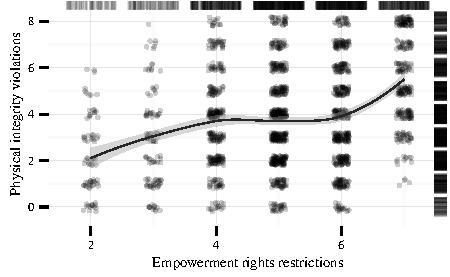
\includegraphics[width=\linewidth]{./sections/02data/scatterRepression.pdf}
\caption[Political repression in authoritarian regimes between 1972 and 2007]{Political repression in authoritarian regimes between 1972 and 2007 with local non-parametric smoother and .95 per cent confidence envelope added.}
\label{fig:scatterRepression}
\end{figure}

The typology of political repression draws out meaningful
differences between authoritarian regimes. This can be seen 
from Figure \ref{fig:scatterRepression} which explores 
their relationship in the unimputed raw data. Here the 
full range of physical integrity violations is observed, 
but empowerment rights restrictions do not take
their lowest possible value $1$. Consequently, all 
authoritarian regimes restrict civil and political 
liberties, but they do not always disrespect the sanctity 
of the individual at the same time. Moreover, Pearson's $r$
between both types of political repression is only  
$0.31$, and the loess smoother gives reason to believe that 
this already weak relationship completely disappears in 
certain regions of the data. More precisely, the smoother 
stays flat across the most densely populated interval of 
empowerment rights restrictions ($4$ to $6$) and no 
inferences whatsoever may be drawn from the level of one 
type of political repression on the other. Thus, there is 
preliminary empirical reason to believe that although 
authoritarian regimes use both types of political 
repression they differ to ``the extent to which they rely 
on one type more than the other'' \citep[336]{Frantz.2014}.

\begin{figure}
\centering
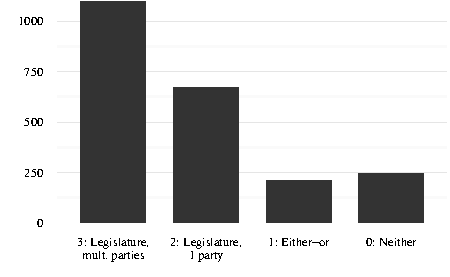
\includegraphics[width=\linewidth]{./sections/02data/barCooptation.pdf}
\caption{Patterns of co-optation in authoritarian regimes between 1972 2007, absolute frequencies.}
\label{fig:barCooptation}
\end{figure}

Frantz and Kendall-Taylor assume that co-optation tips the 
scales of political repression. They measure their key 
explanatory variable by reference to the existence of 
political parties and legislatures. Information on either 
institution is drawn from the `Democracy \& Dictatorship' 
data \citep{Cheibub.2010} which map their de facto 
existence. Frantz and Kendall-Taylor create an index that 
takes the value of 3 if there is a multi-party legislature, 
2 if there is a single-party legislature, 1 if there is no 
legislature but at least one political party or, 
equivalently, if there is a non-partisan legislature, and 0 
if neither exists. Furthermore, the authors presume that 
their index behaves linearly, and they justify their coding
scheme with their interest in the ``interactive effect''
of legislatures and political parties 
\citep[338]{Frantz.2014}. Figure \ref{fig:barCooptation}
explores the empirical picture in the unimputed data. 
The majority of $2,221$ non-missing country-year 
observations falls into the highest category.\footnote{It is
worth noting that this is a post-Cold-War development.} 
Accordingly, more than half of all authoritarian
regimes in the data sponsored multi-party legislatures. 
Single-party regimes come in second, and only a minority of
observations ranks lower than $2$ on the index. In sum, 
empirically speaking almost all authoritarian regimes 
co-opt via some combination of political parties and a 
legislature.

To account for alternative explanations of political repression Frantz and Kendall-Taylor include a large set
of controls. Among these are counts of ongoing civil and 
interstate war as well as event counts of domestic 
political dissent in the form of riots, general strikes, 
and anti-government demonstrations. Moreover, the authors 
include counts of past leadership turnovers and attempted 
coups under the assumption that authoritarian regimes with 
a history of leadership instability are more willing to 
repress. Another set of controls maps socio-economic 
conditions of the regime. For instance, under the 
assumption that oil-revenues offer alternatives to political
repression and institutionalized co-optation Frantz and 
Kendall-Taylor control for oil rents per capita. Moreover, 
since size and growth of the population have been discussed 
as potential causes for state repression in the 
past the authors control for those as well. Moreover, they
add indicators on trade and economic well being as well as
regime type. Finally, following the advice of 
\citet{Carter.2010} cubic splines of leadership duration 
are added to the analyses (c.f. \cite[338]{Frantz.2014}). 
Sample information on these variables are given in the 
appendix.


